\chapter{长时间目标跟踪算法}
周视监控系统需要具备对感兴趣目标进行长时间跟踪的能力。长时间目标跟踪器需要满足以下两个条件:(1)当目标跟丢后,能够重新进行初始化,矫正跟踪误差;(2)当目标暂时离开视野范围,并再次进入视野时,能够再次跟踪。
现有的基于在线学习(online-learning)的目标跟踪器都不能胜任长时间跟踪的任务,因为在线学习的方式存在``漂移''(drift)问题,一旦跟丢,很难重新初始化。在跟踪过程中目标的外观和形状可能会随时发生改变,为了适应目标的动态变化,在线学习机制又是必不可少的。因此,为了实现长时间的目标跟踪,离线的先验知识和在线学习机制都是不可或缺的。第\ref{chap:2}章中实现的基于深度学习的目标检测算法经过大量图像数据的训练,能够在给定图像上可靠地检测感兴趣目标,可以作为目标离线的先验知识来完成目标的初始定位以及跟丢后的重定位。现有的在线式跟踪算法(Struck \cite{struck},KCF \cite{kcf} 等)用来适应目标的动态过程。本文采用一种离线--在线式的方式来实现长时间的目标跟踪,其中离线的基于深度学习的目标检测算法是整个系统得以可靠运行的基石。离线的先验知识于在线学习的过程通过大名鼎鼎P-N learning \cite{p-n} 方法来融合。P-N learning也是广为人知的TLD \cite{tld} 跟踪算法的核心。本文采用Struck算法作为在线的跟踪器。
\section{Struck跟踪算法}

\subsection{Tracking-by-detection方法}
Tracking-by-detection方法之所以如此流行,主要归功于目标检测技术和机器学习技术的快速发展。Tracking-by-detection方法与目标检测方法有着诸多相似之处,近来年目标检测技术的发展突飞猛进,有很多思想和方法可以直接应用到跟踪问题中来。为了应对跟踪对象和背景的外观变化,分类器必须利用分类结果进行在线更新。近年来机器学习技术也有了很大发展,为跟踪过程中分类器在线更新跟踪对象和背景的外观模型打下了基础。

Tracking-by-detection方法在线训练一个分类器,进而将跟踪对象和背景区分开。跟踪过程中,分类器通过在上一帧目标位置的周围搜索最大的分类分值来确定当前帧中目标的位置。一般用滑动窗口的方法来进行搜索。确定了当前帧中目标的位置后,传统的方法是在目标位置的附近采样得到一些有标签的正、负样本,然后用这些样本对分类器进行在线更新。如上所述,传统的方法将分类器在线更新分成两个独立的部分:(1)采样得到一些有标签的训练样本,(2)更新分类器。

用数学语言来描述上述跟踪过程。跟踪器的任务就是在图像帧${f_t} \in F$中估计一个包含跟踪对象的边界框(bounding box)的位置$p \in P$,$t = 1,\dots,T$表示时间。给定一个边界框的位置$p$,我们就可以从边界框
$x_t^p \in X$内的图像块提取特征,然后用分类器对特征进行分类。
经过上述步骤我们就可以得到训练样本集$(x,z)$,其中 $z =  \pm 1$是二元标签,通过$z = sign(h(x))$预测得到,$h:X\rightarrow\textbf{R}$是分类置信函数。然后我们就可以利用这些样本来在线更新分类器。

跟踪过程中,假设当前帧目标的位置可以通过在上一帧目标位置的周围区域最大化$h$来估计。用$p_{t-1}$表示在 时刻估计的边界框位置,跟踪器的任务就是估计一个变换(例如平移)$y_t \in Y$,使得$t$时刻目标的位置为$p_t=p_{t-1}\comp y_t$。$Y$表示搜索空间,它的形式取决于我们要跟踪什么样的运动。在大多数的tracking-by-detection方法中,我们将相邻两帧之间目标对象的运动建模为2D平移运动,即$Y = \left\{ {(u,v)|{u^2} + {v^2} < {r^2}} \right\}$ ,$r$表示搜索半径。$t$时刻相邻两帧之间目标位置的相对变化通过
\begin{equation}
{y_t} = \arg \mathop {\max }\limits_{y \in {Y_t}} h(x_t^{{p_{t - 1}} \comp y})
\end{equation}
来估计,然后跟踪器就可以认为$t$时刻跟踪目标的位置为${p_t} = {p_{t - 1}} \comp {y_t}$。

估计完$t$时刻跟踪目标的位置之后,我们就可以从当前帧获得一组训练样本。我们可以将这一过程分为两个部分:采样和标注。在当前帧估计结果的周围采集$n$个样本
$\left\{ {x_t^{{p_t} \comp y_t^1},\dots,x_t^{{p_t} \comp y_t^n}} \right\}$ 。然后通过某种方法,将这 个样本分别贴上二元标签
$\left\{ {z_t^1,\dots,z_t^n} \right\}$,生成训练样本
$\left\{ {x_t^i,z_t^i} \right\}_{i = 1}^n$。最后,分类器利用这些训练样本进行更新。

下面来详细介绍一下传统的tracking-by-detection方法是如何进行标注工作的。之所以这么做,一方面是为了更加详尽地阐述tracking-by-detection方法的工作原理,另一方面也是为了与Struck跟踪算法进行对比。传统的方法使用相似性度量函数来确定位于${p_t} \comp y_t^i$的样本的标签。给定当前帧跟踪目标的位置$p_t$,相似性度量函数$s(y_t^i,y_t^j;p_t)\in\textbf{R}$确定样本$x_t^{{p_t} \comp y_t^i}$和$x_t^{{p_t} \circ y_t^j}$之间的相似度。我们定义重叠度函数
\begin{equation}
s(y_t^i,y_t^j;{p_t}) = \frac{{({p_t} \circ y_t^i) \cap ({p_t} \circ y_t^j)}}{{({p_t} \circ y_t^i) \cup ({p_t} \circ y_t^j)}}
\end{equation}
来度量两个边界框之间的重叠度。另外一种常用的相似度度量方式是两个边界框中心之间的距离,即 
\begin{equation}
s({y}_t^i,y_t^j;p_t) =  -d(y_t^i,y_t^j)
\end{equation}我们将$y^0$定义为单位变换,即$p=p \comp y^0$,则样本$x_t^{p_t \comp y_t^i}$的标签由标注函数$l(s(y_t^i,y_t^0;{p_t}))$来确定,
\begin{equation}
l(s(y_t^i,y_t^0;{p_t})) = \left\{ \begin{array}{l}

+1 \quad {\rm{for}}\quad s(y_t^i,y_t^0;{p_t}) > {\theta _u}\\

-1 \quad {\rm{for}} \quad s(y_t^i,y_t^0;{p_t}) < {\theta _l}\\

{\rm{\ \ }}0 \quad {\rm{ otherwise}}

\end{array} \right.
\end{equation}
式中$\theta_u$和$\theta_l$分别是标注器的上、下阈值。

\subsection{Tracking-by-detection方法存在的问题}
虽然被广泛研究和使用,tracking-by-detection方法仍然有些问题尚未得到很好的解决。首先,二元分类器的目标是将样本正确地分类,而跟踪器的目的是精确地估计跟踪目标的位置,二者并不是严格一致的。正如S. Hare等 \cite{struck}所指出的,最大的分类置信度并不一定对应最优的目标位置估计。其次,到目前为止我们还不知道该以何种方式进行采样和标注。常用的方法是根据样本到目标位置的距离来决定它是正样本还是负样本。显然,这种方法不可避免地会引入一些样本噪声。因此,最近几年提出了一些算法专门研究如何提高分类器对样本噪声的鲁棒性,其中包括半监督学习 \cite{boost-track} \cite{multi-view},多实例学习 \cite{mil} \cite{mib}等。
传统的tracking-by-detection方法,需要启发式地从当前帧目标位置的周围采集正、负样本,来进行分类器的更新。虽然上文中提到的半监督学习和多实例学习等方法能够增加分类器对样本噪声的鲁棒性,但是都没有从根本上解决问题。真正的问题是:我们将采样和分类器的训练看成是两个级联的、相互独立的过程。采样和分类器的训练应该是相互影响、同时进行的。为了避免启发式的采样过程(需要对目标位置的估计很精确),人们提出了两种解决方案。一种是基于结构化支持向量机(Structural SVM)\cite{struck},另一种是是基于Ranking SVM \cite{rank-svm}。这两种方法的核心思想都是将样本之间的结构约束(例如相对排序和区域重叠度)集成到大间隔优化问题中去。支持向量机(SVM)具有泛化能力强、对样本噪声不敏感等优点,而且核函数的使用使输入向量表达的特征更加丰富。结构化输出支持向量机是二元支持向量机的一种泛化形式,能够处理例如图、树等复杂的输出结构。合理地利用输出空间中不同输出之间的关系,我们能够从训练样本中得到更多的信息。因此,本文采用基于结构化输出支持向量机(structural output support vector machine)的方法来进行跟踪。在本文中,输出空间中的元素是由4个坐标(上、下、左、右)确定的边界框。

\subsection{Struck跟踪算法}
与传统的tracking-by-detection方法不同的是,基于Structural SVM的跟踪算法将跟踪问题看作一个结构化预测问题:预测包含跟踪目标的边界框,而不是一个二元分类问题。在下文中,我们将会看到如何在结构学习的框架中表述视频目标跟踪问题。

\subsubsection{结构化输出支持向量机}
结构化预测的目的就是,对于一个给定的输入$x \in X$,预测对应的结构化输出$y \in Y$。给定一组输入图像$\left\{x_1,\dots,x_n\right\} \subset X$和它们对应的标签$\left\{y_1,\dots,y_n\right\} \subset Y$,希望能够学习一个映射$g:X \rightarrow Y$用于完成结构化预测。这里$Y=\left\{(t,l,b,r)|(t,l,b,r) \in \textbf{R}^4\right\}$,$(t,l,b,r)$用于表示边界框的4个坐标,在结构学习的框架下学习映射$g$
\begin{equation}
g(x)=\arg \max_{y \in Y}{f(x,y)}
\end{equation}
$f(x,y)$是一个判别函数,样本$(x,y)$中输入$x$和输出$y$越是匹配,函数$f$的值就越大。因此结构学习的任务就是学习判别函数$f$。

为了学习判别函数$f$,Struck使用下述泛化的支持向量机
\begin{equation}
\begin{aligned}
& \min_{\omega,\zeta} &&\frac{1}{2}\|\omega\|^2 + C\sum_{i=1}^{n}\zeta_i\\
& s.t.&&\langle \omega,\phi(x_i,y_i)\rangle-\langle\omega,\phi(x_i,y)\rangle \geq \Delta(y_i,y)-\zeta_i,\quad \forall i,\forall y\in Y\\
\end{aligned}
\end{equation}
式中$f(x_i,y)=\langle\omega,\phi(x_i,y)\rangle$,$\phi(x_i,y)$是一个联合映射核,根据核函数的性质可知下式成立
\begin{equation}
k((x,y),(x',y'))=\langle\phi(x,y),\phi(x',y')\rangle
\end{equation}
这一优化问题的约束条件保证$f(x_i,y_i)$比任意$f(x_i,y)$至少大$\Delta(y_i,y)$,与二元支持向量机类似,这也是大间隔分类思想的体现。正是这种大间隔分类的作用,判别函数$f$具有很强的判别能力。损失函数应该满足当且仅当$y=y_i$时$\Delta(y_i,y)=0$,而且当$y_i$变得和$y$越来越相似时,$\Delta(y_i,y)$趋近于0。损失函数在本文提出的算法中至关重要,它可以解决上文中提到的tracking-by-detection方法将所有训练样本同等对待的问题。

\subsubsection{损失函数的选取}
Struck中损失函数$\Delta(y_i,y)$定义为
\begin{equation}
\Delta(y_i,y)=1-{\rm{IoU}}(y_i,y)
\end{equation}
该函数满足:(1)当且仅当$y$和$y_i$相同时,损失函数$\Delta(y_i,y)=0$;(2)当$y$和$y_i$不重叠时,损失函数$\Delta(y_i,y)=1$。

\section{P-N learning}
PN learning, P指代Positive Constraint,也称之为P-expert或者growing event,N指代Negative Constraint,也称之为N-expert或者pruning event。
P-expert的作用是发现目标的新的外观(形变),并以此来增加正样本的数量,从而使得检测模块更具鲁棒性;
N-expert的作用是生成负的训练样本。N-expert的前提假设是,(被跟踪的)前景目标仅可能出现在视频帧中的一个位置,因此,如果前景目标的位置是确定的,那么其周围必然是负样例。 PN学习包含四个部分:(1)一个待学习的分类器;(2)训练样本集--一些已知类别标签的样本;(3)监督学习--一种从训练样本集中训练分类器的方法;(4)P-N experts--在学习过程中用于产生正(训练)样本和负(训练)样本的表达函数;这四个部分之间的关系如图 \ref{fig:pn-learning}所示。
\begin{figure}[h]
	\centering
	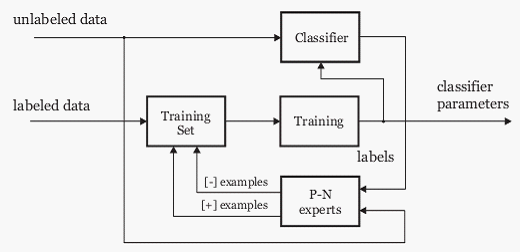
\includegraphics[width=\textwidth]{pn-learning}
	\caption{P-N learning示意图。}
	\label{fig:pn-learning}
\end{figure}
从理论上分析得出,只要P-expert和N-expert预测的准确率超过50\%就能够提高分类器的性能,因此本文中的P-expert和N-expert选用基于深度学习的目标检测算法,经过实验证明该算法预测的正确率远远超过50\%,能够纠正在线学习所导致的漂移的问题。

\section{实验结果及分析}
在线学习算法及P-N learning融合过程运行在Intel I7处理器上,基于深度学习的目标检测算法运行在Nvidia Titan X上,二者之间通过Tcp/IP协议交换数据,由于基于深度学习的目标检测对一幅图像需要230ms,因此P-N learning融合的过程隔几桢做一次,但实验证明这对跟踪效果没有明显影响。典型的图像序列跟踪效果如图 \ref{fig:track-result} 所示。
\begin{figure}
	\subfigure[David]{
		\includegraphics[width=8cm, height=4cm]{david}
	}
	\subfigure[Sylvester] {
		\includegraphics[width=8cm, height=4cm]{syl}
	}
	\subfigure[Woman] {
		\includegraphics[width=8cm, height=4cm]{woman}
	}
	\subfigure[Car] {
		\includegraphics[width=8cm, height=4cm]{car}
	}
	\subfigure[Girl] {
		\includegraphics[width=8cm, height=4cm]{girl}
	}
	\subfigure[Faceocc] {
		\includegraphics[width=8cm, height=4cm]{faceocc}
	}
	\caption{在典型图像序列上的跟踪效果}
\end{figure}